\documentclass{article}
\usepackage{amsmath}
\usepackage{float}
\usepackage{graphicx}


\title{Linear Regression}
\author{Ta Quang Minh}
\date{\today}

\begin{document}

\maketitle

\section{Introduction}
Linear regression is one of the most fundamental and widely used statistical techniques in data analysis and machine learning. It serves as a foundational tool for modeling the relationship between a dependent variable and one or more independent variables. In this report, we aim to provide a comprehensive overview of linear regression, covering its principles, applications, advantages, limitations, and variations.

\section{Mathematical Formulation}

In the context of machine learning, linear regression is a supervised learning algorithm used for regression tasks. The input to a linear regression model consists of the independent variables \( x_1, x_2, ..., x_n \), and the output is the predicted value of the dependent variable \( y \).

Linear regression assumes a linear relationship between the independent variables (predictors) and the dependent variable (response). The relationship is expressed through a linear equation:
\begin{equation}
    Y = \beta_0 + \beta_1X_1 + \beta_2X_2 + \ldots + \beta_nX_n + \epsilon
\end{equation}
Where:
\begin{itemize}
    \item $Y$ is the dependent variable.
    \item $X_1, X_2, \ldots, X_n$ are the independent variables.
    \item $\beta_0, \beta_1, \ldots, \beta_n$ are the coefficients.
    \item $\epsilon$ is the error term.
\end{itemize}


Let's denote:
\begin{itemize}
    \item $Y_i$ as the observed value of the dependent variable for the $i$-th observation.
    \item $\hat{Y}_i$ as the predicted value of the dependent variable for the $i$-th observation.
    \item $X_{i1}, X_{i2}, \ldots, X_{in}$ as the values of the independent variables for the $i$-th observation.
\end{itemize}

The predicted value of the dependent variable $\hat{Y}_i$ for the $i$-th observation can be calculated as:
\begin{equation}
    \hat{Y}_i = \beta_0 + \beta_1 X_{i1} + \beta_2 X_{i2} + \ldots + \beta_n X_{in}
\end{equation}

The error term $\epsilon_i$ for the $i$-th observation is the difference between the observed value $Y_i$ and the predicted value $\hat{Y}_i$:
\begin{equation}
    \epsilon_i = Y_i - \hat{Y}_i
\end{equation}

The goal is to find the values of the coefficients ($\beta_0, \beta_1, \ldots, \beta_n$) that minimize the sum of squared errors (SSE) as the loss function:
\begin{equation}
    \text{SSE} = \sum_{i=1}^{N} \epsilon_i^2
\end{equation}
Where $N$ is the total number of observations.

The optimal value for the coefficients of linear regression can be calculated by letting the gradient of the loss function be 0. It therefore can be calculated by the close-formed formula :

\[
\boldsymbol{\beta} = (\mathbf{X}^T \mathbf{X})^{-1} \mathbf{X}^T \mathbf{Y}
\]

Where:
\begin{itemize}
    \item $\boldsymbol{\beta}$ is the vector of coefficients.
    \item $\mathbf{X}$ is the matrix of independent variables (also known as the design matrix), with each row representing an observation and each column representing a different variable.
    \item $\mathbf{Y}$ is the vector of dependent variable values.
\end{itemize}

Another approach on finding the optimal coefficients involved applying gradient descent on the loss function.

\section{Implementation on real data}
\subsection{Example 1}
In this example, we analyze a dataset generated using a linear relationship between an independent variable \( X \) and a dependent variable \( y \). The dataset consists of 100 samples with one feature.

The independent variable \( X \) is generated using NumPy's random number generator with values ranging from 0 to 10. The dependent variable \( y \) is generated using a linear relationship with some added Gaussian noise. Specifically:

The dependent variable \( y \) is generated using the equation of a line with added Gaussian noise:
\[
y_i = \text{{true\_slope}} \times X_i + \text{{true\_intercept}} + \text{{noise}}
\]
Where:
\begin{itemize}
    \item \text{{true\_slope}} is the true slope of the linear relationship.
    \item \text{{true\_intercept}} is the true intercept of the linear relationship.
    \item \text{{noise}} is Gaussian noise with mean 0 and standard deviation 2.
\end{itemize}

The true parameters used to generate the data are as follows:
\begin{itemize}
    \item True Slope (\( \beta_1 \)): \( 3.5 \)
    \item True Intercept (\( \beta_0 \)): \( 10.0 \)
\end{itemize}

To assess the performance of the linear regression model, we split the dataset into training and testing sets. 80\% of the data is used for training and a smaller portion 20\% for testing.

Using gradient descent on the training set, the algorithm was able to estimate the coefficient as 3.4961039 and 10.41267872. It result in this regression line:

\begin{figure}[H]
    \centering
    \resizebox{\textwidth}{!}{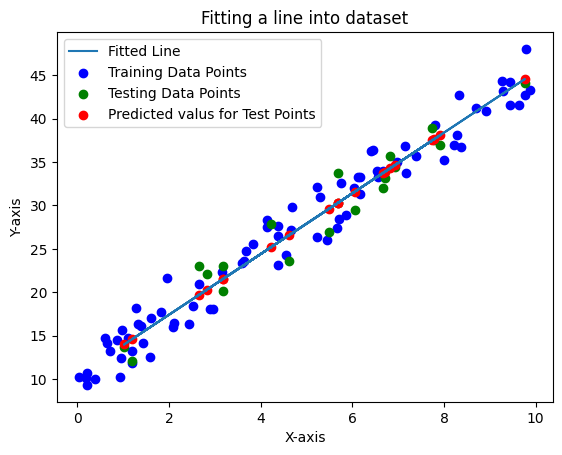
\includegraphics{linear1.png}}
    \caption{Linear regression on 1D input}
    \label{fig:example}
\end{figure}

The error of the prediction is calculated to be:

Mean Squared Error (MSE): 3.6710131285311975

Root Mean Squared Error (RMSE): 1.9159888122145174

\subsection{Example 2}

In this example, the dependent variable \( y \) is also generated using the linear combination of independent variables x1 and x2 with added Gaussian noise:
\[
y_i = \text{{true\_slope1}} \times X_{1i} + \text{{true\_slope2}} \times X_{2i} + \text{{true\_intercept}} + \text{{noise}}
\]
Where:
\begin{itemize}
    \item \text{{true\_slope1}} and \text{{true\_slope2}} are the true slopes of the linear relationship for \( X_1 \) and \( X_2 \) respectively.
    \item \text{{true\_intercept}} is the true intercept of the linear relationship.
    \item \text{{noise}} is Gaussian noise with mean 0 and standard deviation 2.
\end{itemize}

The true parameters used to generate the data are as follows:
\begin{itemize}
    \item True Slope for \( X_1 \) (\( \beta_1 \)): \( 2.0 \)
    \item True Slope for \( X_2 \) (\( \beta_2 \)): \( 1.5 \)
    \item True Intercept (\( \beta_0 \)): \( 5.0 \)
\end{itemize}

Feeding it into the regression model, we obtain the following regression plane:

\begin{figure}[H]
    \centering
    \resizebox{\textwidth}{!}{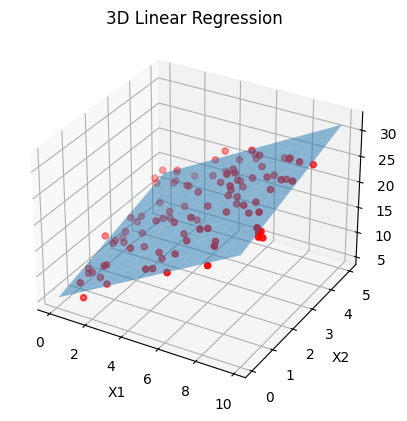
\includegraphics{linear2.png}}
    \caption{Linear regression on 2D input}
    \label{fig:example}
\end{figure}

The model estimate the coefficients to be 1.92239569, 1.47812891 and  5.19213193 respectively.

\section{Applications of Linear Regression}
Linear regression finds application in various fields including finance, economics, biology, social sciences, and engineering. Some common applications include:
\begin{enumerate}
    \item \textbf{Predictive Modeling:} Predicting sales figures, stock prices, or housing prices based on historical data.
    \item \textbf{Trend Analysis:} Analyzing trends and patterns in data to make informed decisions.
    \item \textbf{Risk Assessment:} Assessing risk factors and predicting outcomes in insurance and finance.
    \item \textbf{Marketing Analysis:} Understanding the impact of marketing campaigns on sales and customer behavior.
\end{enumerate}

\section{Advantages of Linear Regression}
Linear regression offers several advantages:
\begin{itemize}
    \item \textbf{Simplicity:} Linear regression is easy to understand and interpret, making it accessible to a wide range of users.
    \item \textbf{Efficiency:} It can handle large datasets efficiently, making it suitable for big data analytics.
    \item \textbf{Interpretability:} The coefficients in linear regression provide insights into the relationship between variables.
\end{itemize}

\section{Limitations of Linear Regression}
Despite its advantages, linear regression has some limitations:
\begin{itemize}
    \item \textbf{Linearity Assumption:} Linear regression assumes a linear relationship between variables, which may not hold true in all cases.
    \item \textbf{Sensitivity to Outliers:} Linear regression is sensitive to outliers, which can significantly affect the model's performance.
    \item \textbf{Multicollinearity:} When independent variables are highly correlated, it can lead to multicollinearity issues, affecting the model's stability and interpretability.
\end{itemize}

\section{Variations of Linear Regression}
There are several variations of linear regression:
\begin{enumerate}
    \item \textbf{Simple Linear Regression:} Involves a single independent variable.
    \item \textbf{Multiple Linear Regression:} Involves multiple independent variables.
    \item \textbf{Polynomial Regression:} Fits a polynomial curve to the data.
    \item \textbf{Ridge Regression:} Addresses multicollinearity by adding a penalty term to the regression coefficients.
    \item \textbf{Lasso Regression:} Similar to Ridge regression but uses the L1 regularization penalty.
    \item \textbf{Elastic Net Regression:} Combines the penalties of Ridge and Lasso regression.
\end{enumerate}

\section{Conclusion}
In this report, we have presented an overview of Linear regression, as well as its variants, applications, advantages, and limitations.
It is a powerful statistical technique with widespread applications across various domains. While it has its limitations, its simplicity, efficiency, and interpretability make it an indispensable tool for data analysis and predictive modeling.

Understanding the principles, applications, and variations of linear regression is essential for leveraging its full potential in real-world scenarios.

\end{document}
